\chapter{Storage}

\framedt{Data Loss}{
   \textit{``Storage is crucial because, if a switch fails, or a server fails, the service will be interrupted, but the data will still be there. \ul{If the storage fails, the \textbf{data will be lost}}.''}
   -Prof. Cisternino\\

   \textbf{Data} is the most important of a system. Since data loss is \textbf{permanent}, the storage is completely different from computing or networking.
}

\begin{paracol}{2}
   \colfill
   Historically the storage was the slowest part of the system, \textit{ms} against \textit{ns} of the CPU.
   Today, with SSDs, the gap is considerably reduced to \textit{$\mu s$}, they are $\sim 100x$ times faster.
   
   \ul{NVMe stands for \textit{Non-Volatile Memory Express}, and is a protocol (\textit{not a HW component!})} that allows to access the storage directly from the PCIe bus, without having to go through the SATA controller. This allows to have a much higher throughput, and a much lower latency.

   \note{Optane was a technology developed by intel which is now end of life}

   \colfill
   \switchcolumn

   \begin{figure}[htbp]
      \centering
      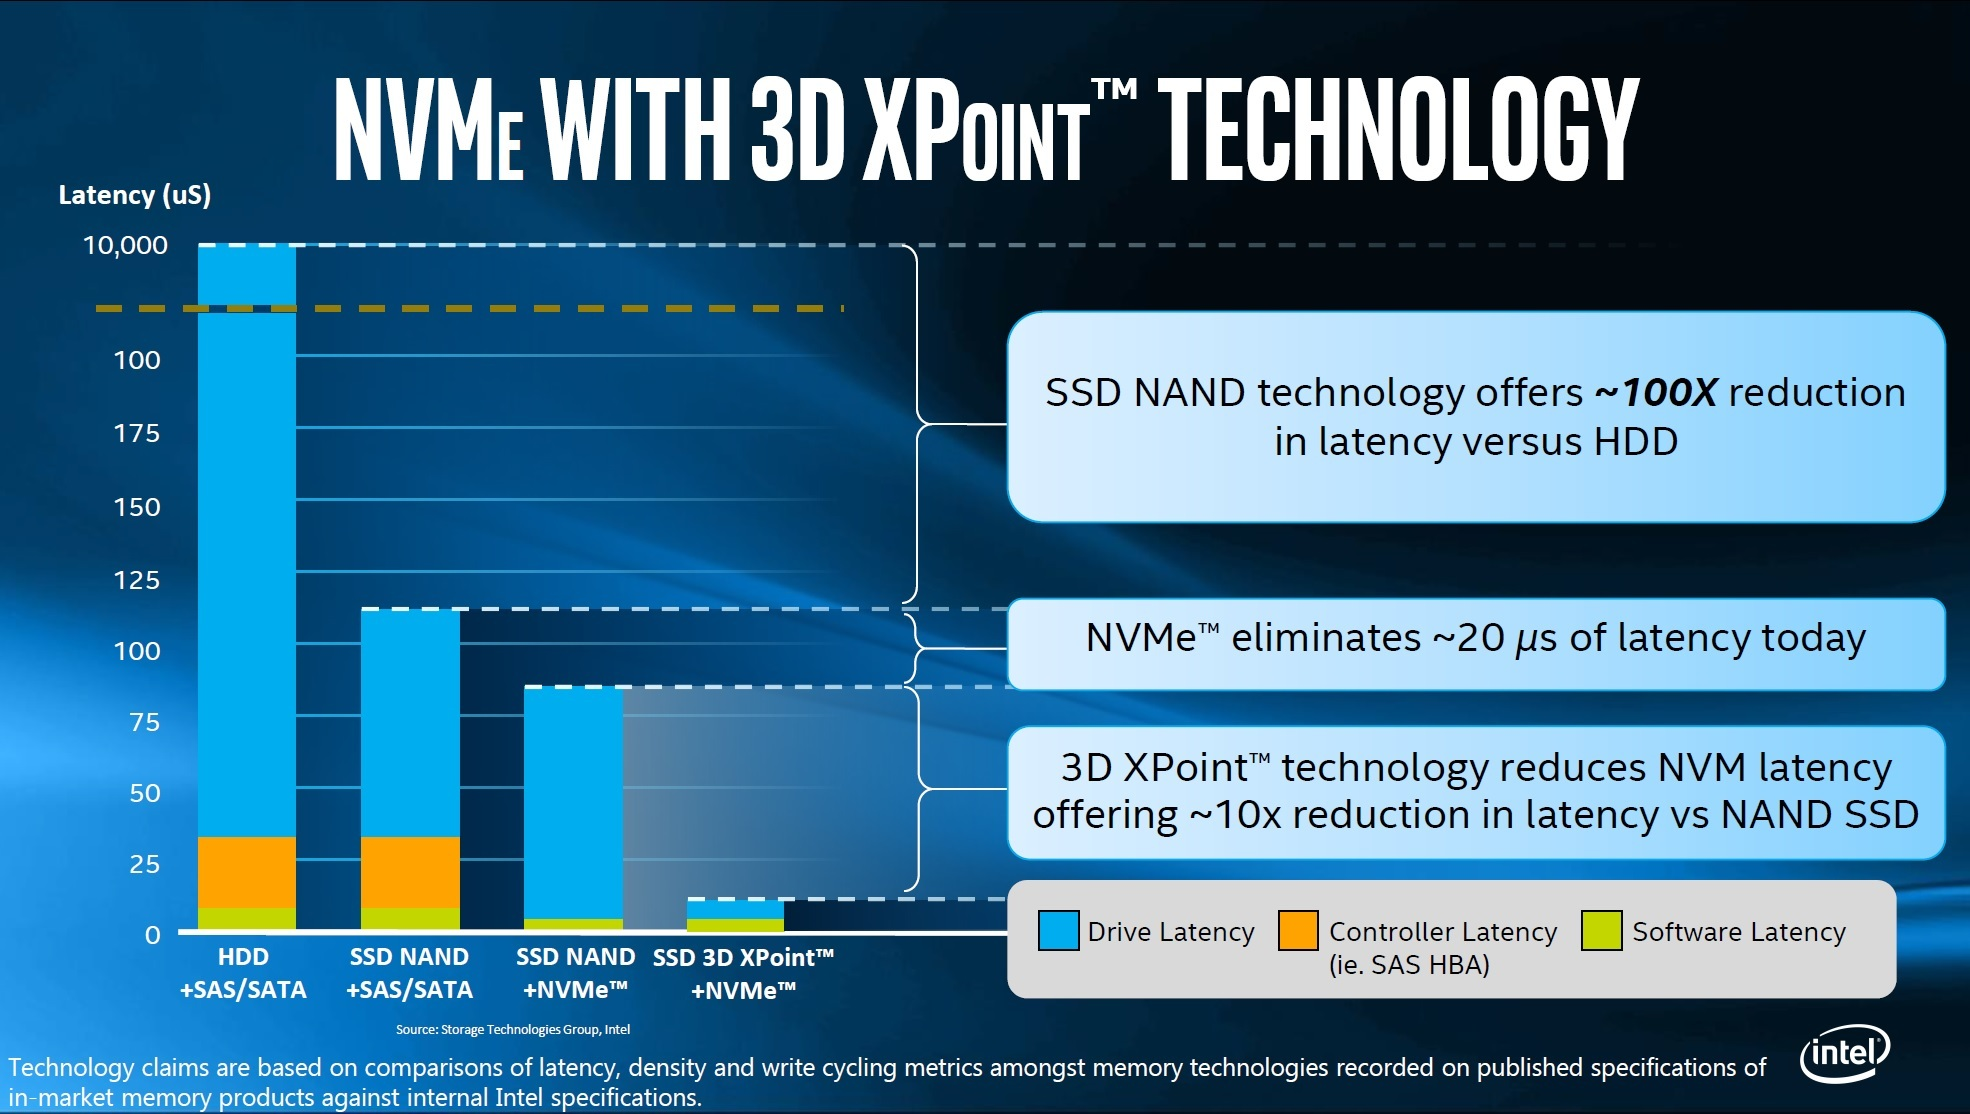
\includegraphics{images/storage_intel.jpg}
      \caption{Storage types comparison}
      \label{fig:storage_intel}
      NVMe basically removes the orange part of the figure, which is the latency introduced by the controller, since it is a \textit{controller-less protocol} and allows to access the storage directly from the PCIe bus.
   \end{figure}
\end{paracol}


\framedt{
   \textit{Why would a 15TB disk be better than a 27TB disk?}\\
   }{
      \note{Assume the same performance, and the same price.}
      It would be preferrable because \ul{it would take less time to extract all the data from the disk}\footnotemark[1], since it is smaller.
      
      However, large capacity drives are used for \textit{cold storage}, where the data is not accessed frequently, speed is not a priority, and even if the data is accessed, only a portion of the disk is needed at a time; in case of failure and thus needing to retrieve an entire backup, the time taken to retrieve the data is not a priority, since this ---hopefully--- happens only ``once''.
      }
      
\footnotetext[1]{i.e. taking advantage of the space provided}
\section{SSDs - QLC and TLC}
SSDs were invented by Toshiba back in 1980, but they were not popular for almost 30 years, until they eventually became cost-effective. Sometimes extra size in SSDs is used for redundancy, to increase the lifespan of the disk e.g. on a 30TB disk, only 10TB are used, the rest is used for redundancy, extending x3 the lifespan of the disk.

\note{DWPD stands for \textit{Drive Writes Per Day}, and is a measure of how many times the disk can be written to in a day. It can be calculated as $\frac{TBW}{365\times\textit{Years of Warranty}\times\textit{capacity}}$}.

TLC stands for \textit{Triple Level Cell}, and QLC stands for \textit{Quad Level Cell}. The difference between the two is the number of bits stored in each cell. The more bits stored in each cell, the cheaper the disk is, but the slower it is. The more bits stored in each cell, the more difficult it is to read and write the data, and the more difficult it is to keep the data stored in the cell.

Generally QLC disks are used for cold storage, while TLC disks are used for hot storage.
TLC in general is more reliable than QLC, has a longer lifespan and better performance, however they cost more.

\section{Storage Concepts}
\subsection{Tiering - Memory Hierarchy}

\begin{figure}[htbp]
   \centering
   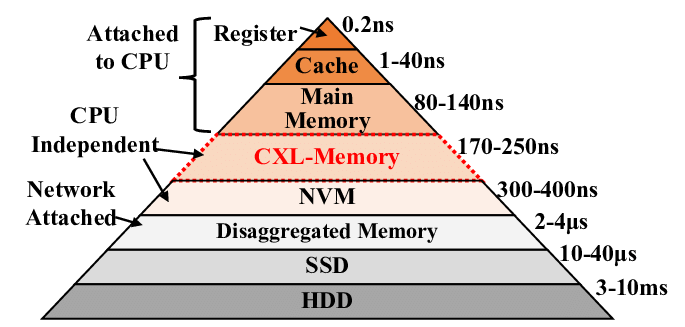
\includegraphics{images/tiering_memory.png}
   \caption{Memory tiering hierarchy}
   Ram could actually be split in \texttt{RAM} and \texttt{nvRAM} (Non-volatile \texttt{RAM}, uses \texttt{nvDIMM}), which is used to store the data in case of a power failure.
   Sometimes, \textit{tape} is included in the hierarchy, because it is used for long-term storage, and it is very cheap.
   \label{fig:tiering_memory}
\end{figure}

Tiering consists in categorizing the data in different categories, and storing the data in different types of storage, depending on the category. The data that is accessed more frequently is stored in the fastest storage, while the data that is accessed less frequently is stored in the slowest storage. This allows to increase the performance, and to reduce the cost. 

\subsection{IO operations, are they all the same?}
\textbf{IOPS} (Input/output operations per second) is an input/output
performance metric used to characterize computer storage devices; it is associated with an access pattern: \textit{random} or \textit{sequential}.

\subsubsection{Random vs Sequential access}

Before explaining the distinction, is important to remember the concept of \textit{queues}: for each thread, the OS can implement a series of queues to solve asynchronously the I/O requests. Using multiple queue can make performances better, since having
the OS to manage parallel requests will increase throughput.
If the queries are latency sensible, not using a queue is better, since
it allows a single query to have ``max'' priority.

\textit{Random access files} are advantageous in scenarios where frequent direct access or modification of specific records is required, while \textit{sequential access files} are advantageous in scenarios where frequent reads of the full files are required. The disk behaves differntly in case of access of those files.

To have a full picture of random vs sequential access, check this site: \url{https://www.prepbytes.com/blog/general/difference-between-sequential-and-random-access-file/} 

\newpage
\subsubsection{Cisternino's demo}
Prof. Cisternino showed a demo in class, where he used a tool to measure the IOPS of a disk.
\begin{figure}[htbp]
   \centering
   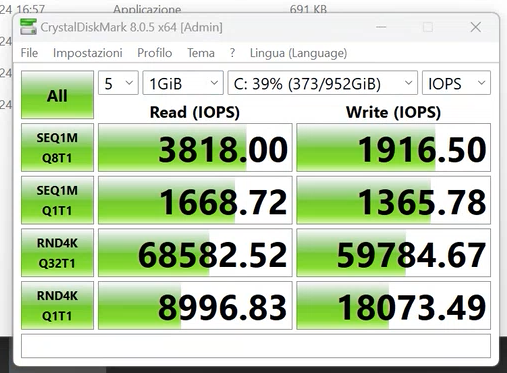
\includegraphics{images/iops.png}
   \caption{IOPS demo; respetively}
   \label{fig:iops}
\end{figure}

\ul{Recall that IOPS by itself is meaningless!} It is a number that must qualified and put in relationship with something else.

\subsection{Latency and Storage Aggregation}
A mechanical hard drive introduces 2.71\% of latency when reading, for instance, 40MB of data.  Optane can perform 416 accesses in the same time needed by a mechanical hard drive to perform 1 access. It looks like the latency in this latter case is neglegtible. Someone may be tempted to reduce the size of read/write operations and perform multiple smaller ones, since ``it's free''. 

Latency in general is due to:
\begin{itemize}
   \item \textbf{Software}\\
   $\mu s$ order which cannot be removed
   \item \textbf{Controller}\\
   Taken down to $20\mu s$ with NVMe (even $2.8\mu s$ according to Copilot)
   \item \textbf{HDD latency}\\
   This was drastically reduced with SSDs and got even less with 3D NAND.
\end{itemize}
Latency may be solved by \textbf{storage aggregation}, which consists in aggregating multiple storage devices into a single logical unit, in order to increase the performance and reliability.
Even if the data is split in multiple disks, the whole system is ``pictured'' as a single huge drive\footnote{\textit{``Cloud resource pooling''} rings a bell?}, making a huge difference in terms of latency, since multiple \texttt{read/write} requests may be sent in parallel to multiple disks.

\newpage
\subsection{Storage Fabric - Fibre Channel}
\textbf{Fibre Channel} is the fabric dedicated to storage; the link coming from the storage ends up in the \textit{HBA} (Host Bus Adapter) in the server.
\begin{paracol}{2}

   \colfill
   The idea is to have an interface which announces itself as drive and that manages the remote storage through Fibre Channel.
   Fibre Channel typically runs on optical fiber cables, but may also run on Ethernet cables (FCoE).

   In Fig. \ref{fig:fibrechannel} is depicted the ideal architecture for Fibre Channel, where the storage is connected to the network through a switch, and the servers have a dedicated HBA to connect to the storage.
   \colfill
   
   \switchcolumn
   \begin{figure}[htbp]
      \centering
      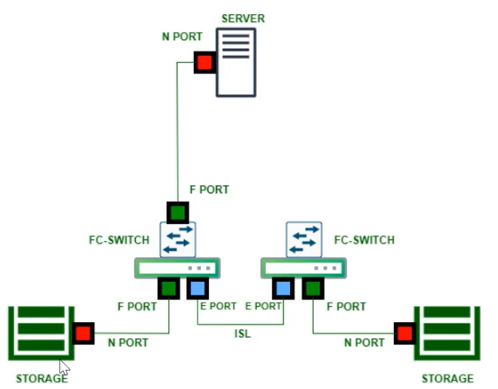
\includegraphics{images/fibrechannel.png}
      \caption{Fibre Channel desired architecture}
      \label{fig:fibrechannel}
   \end{figure}
   
\end{paracol}

\begin{figure}[htbp]
   \centering
   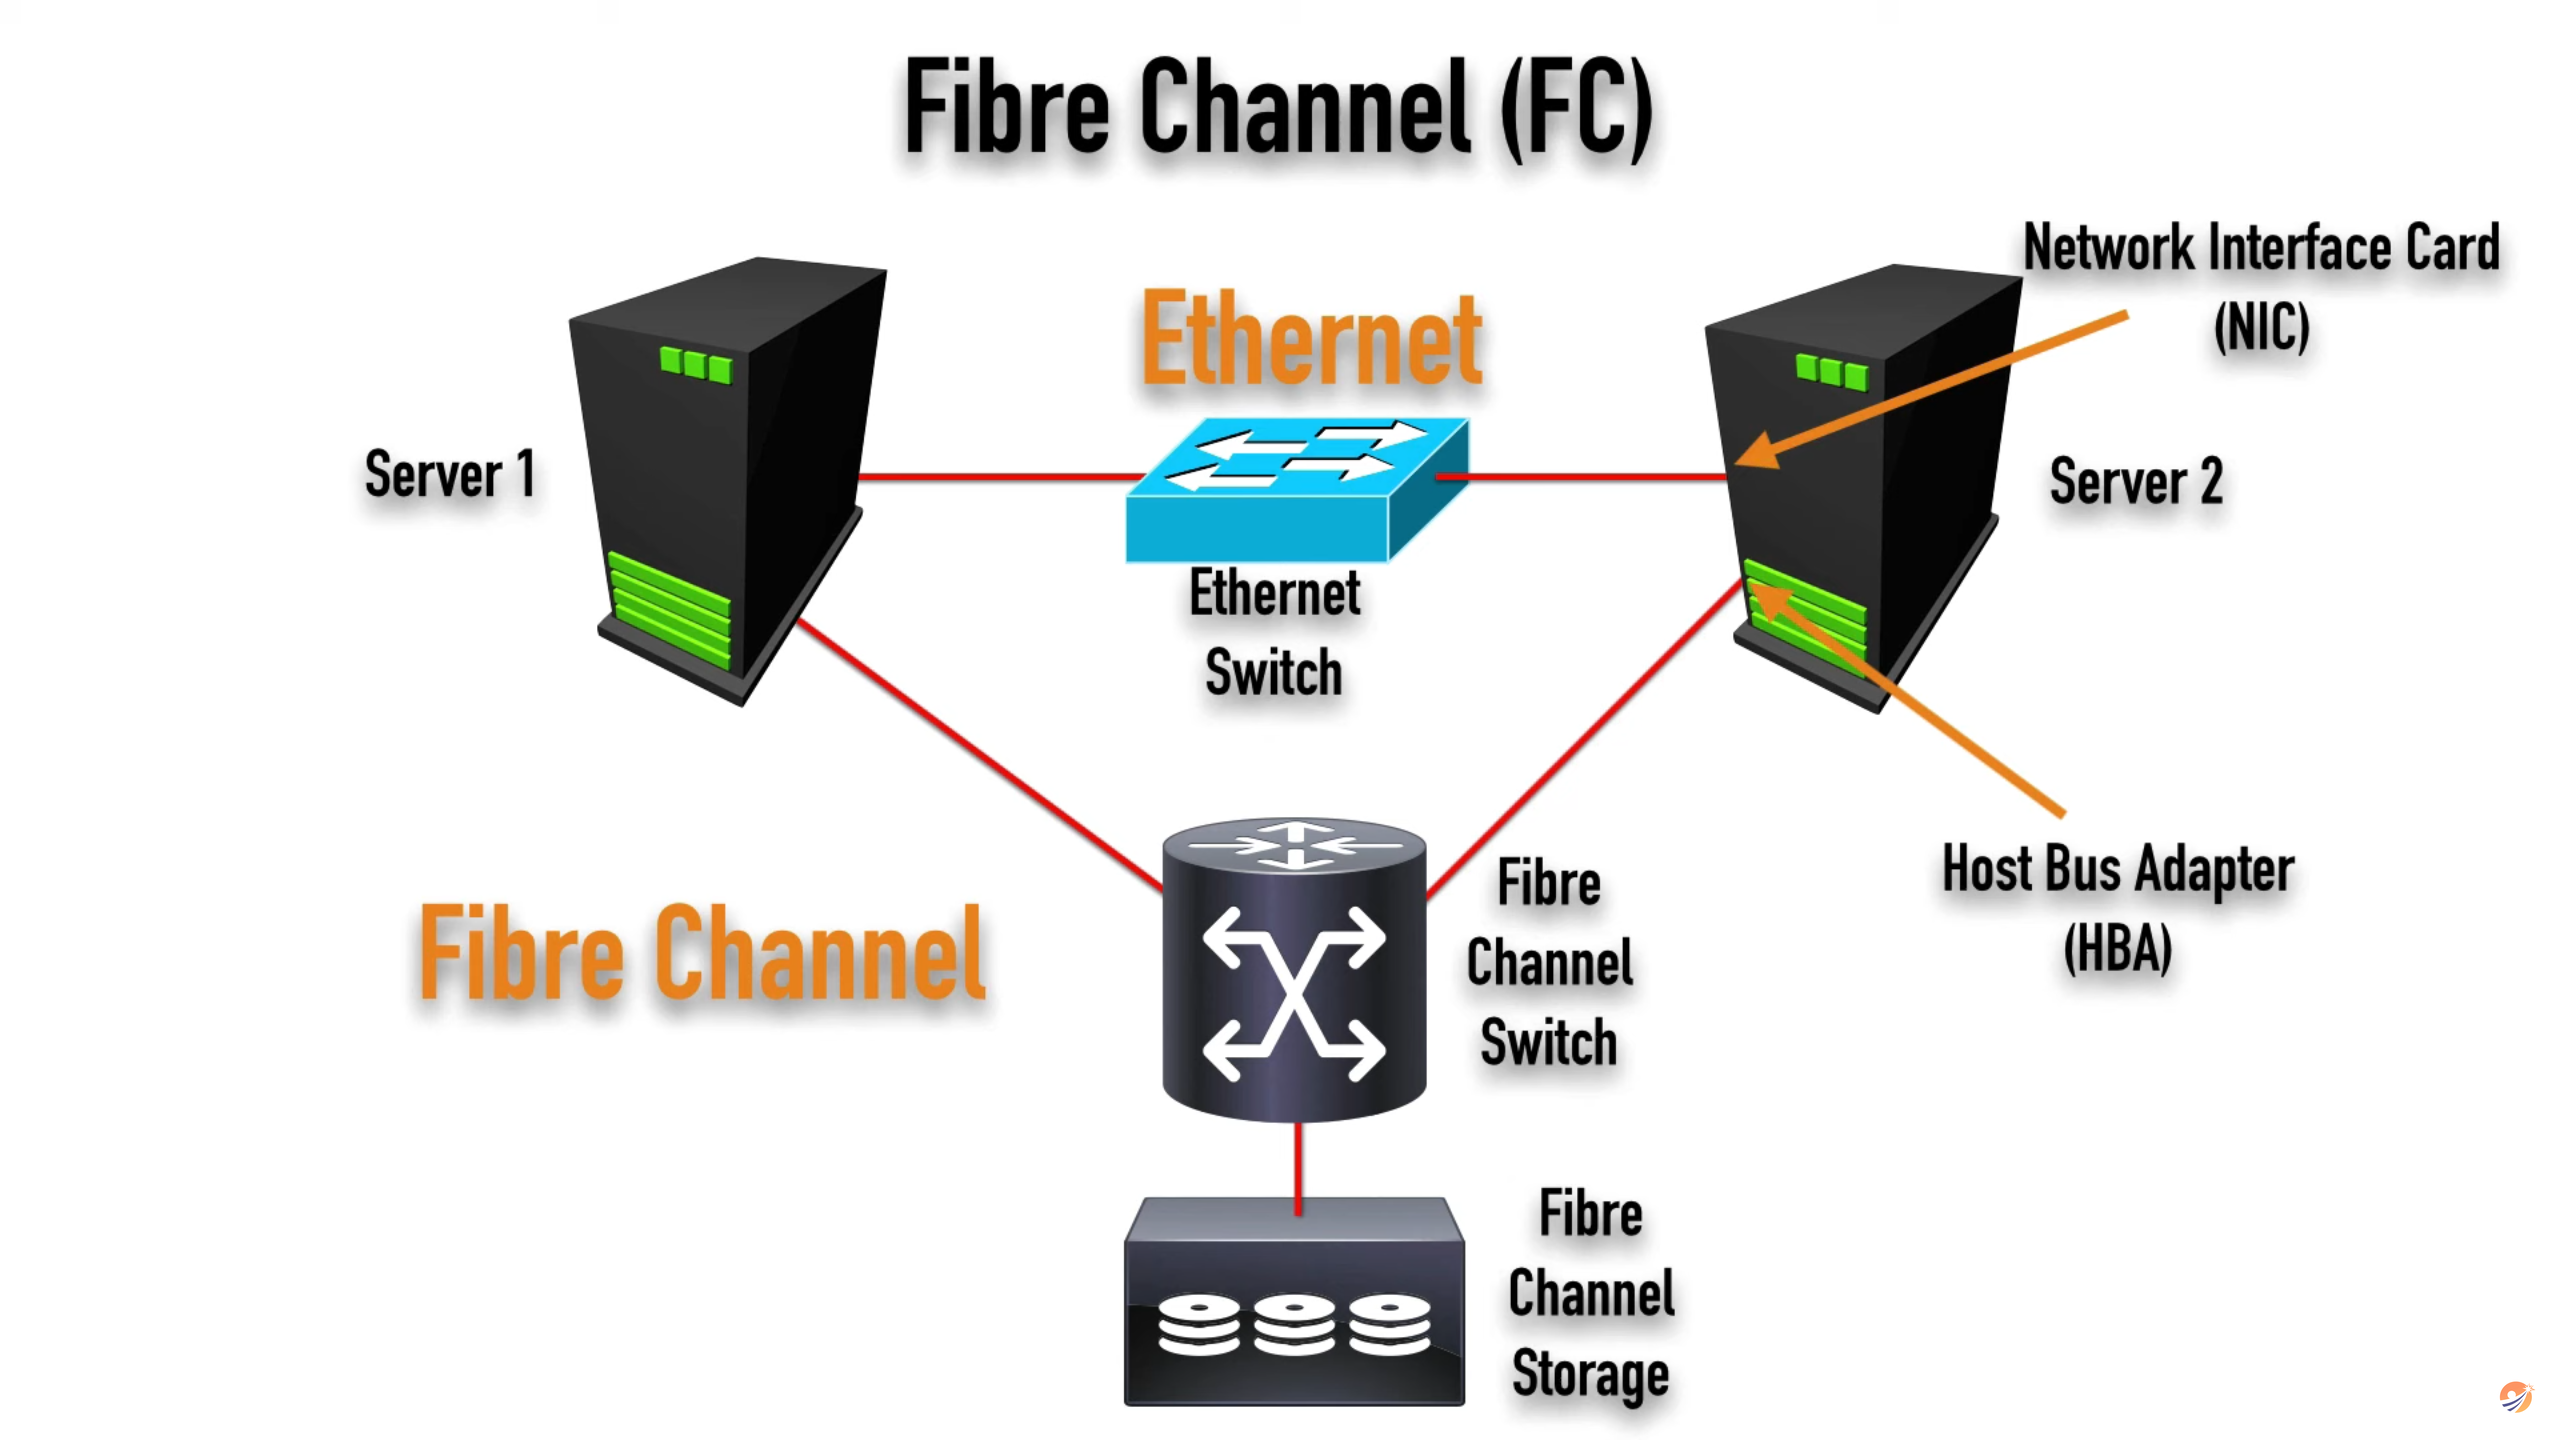
\includegraphics[width=0.32\columnwidth]{images/storage_fabric1.png}
   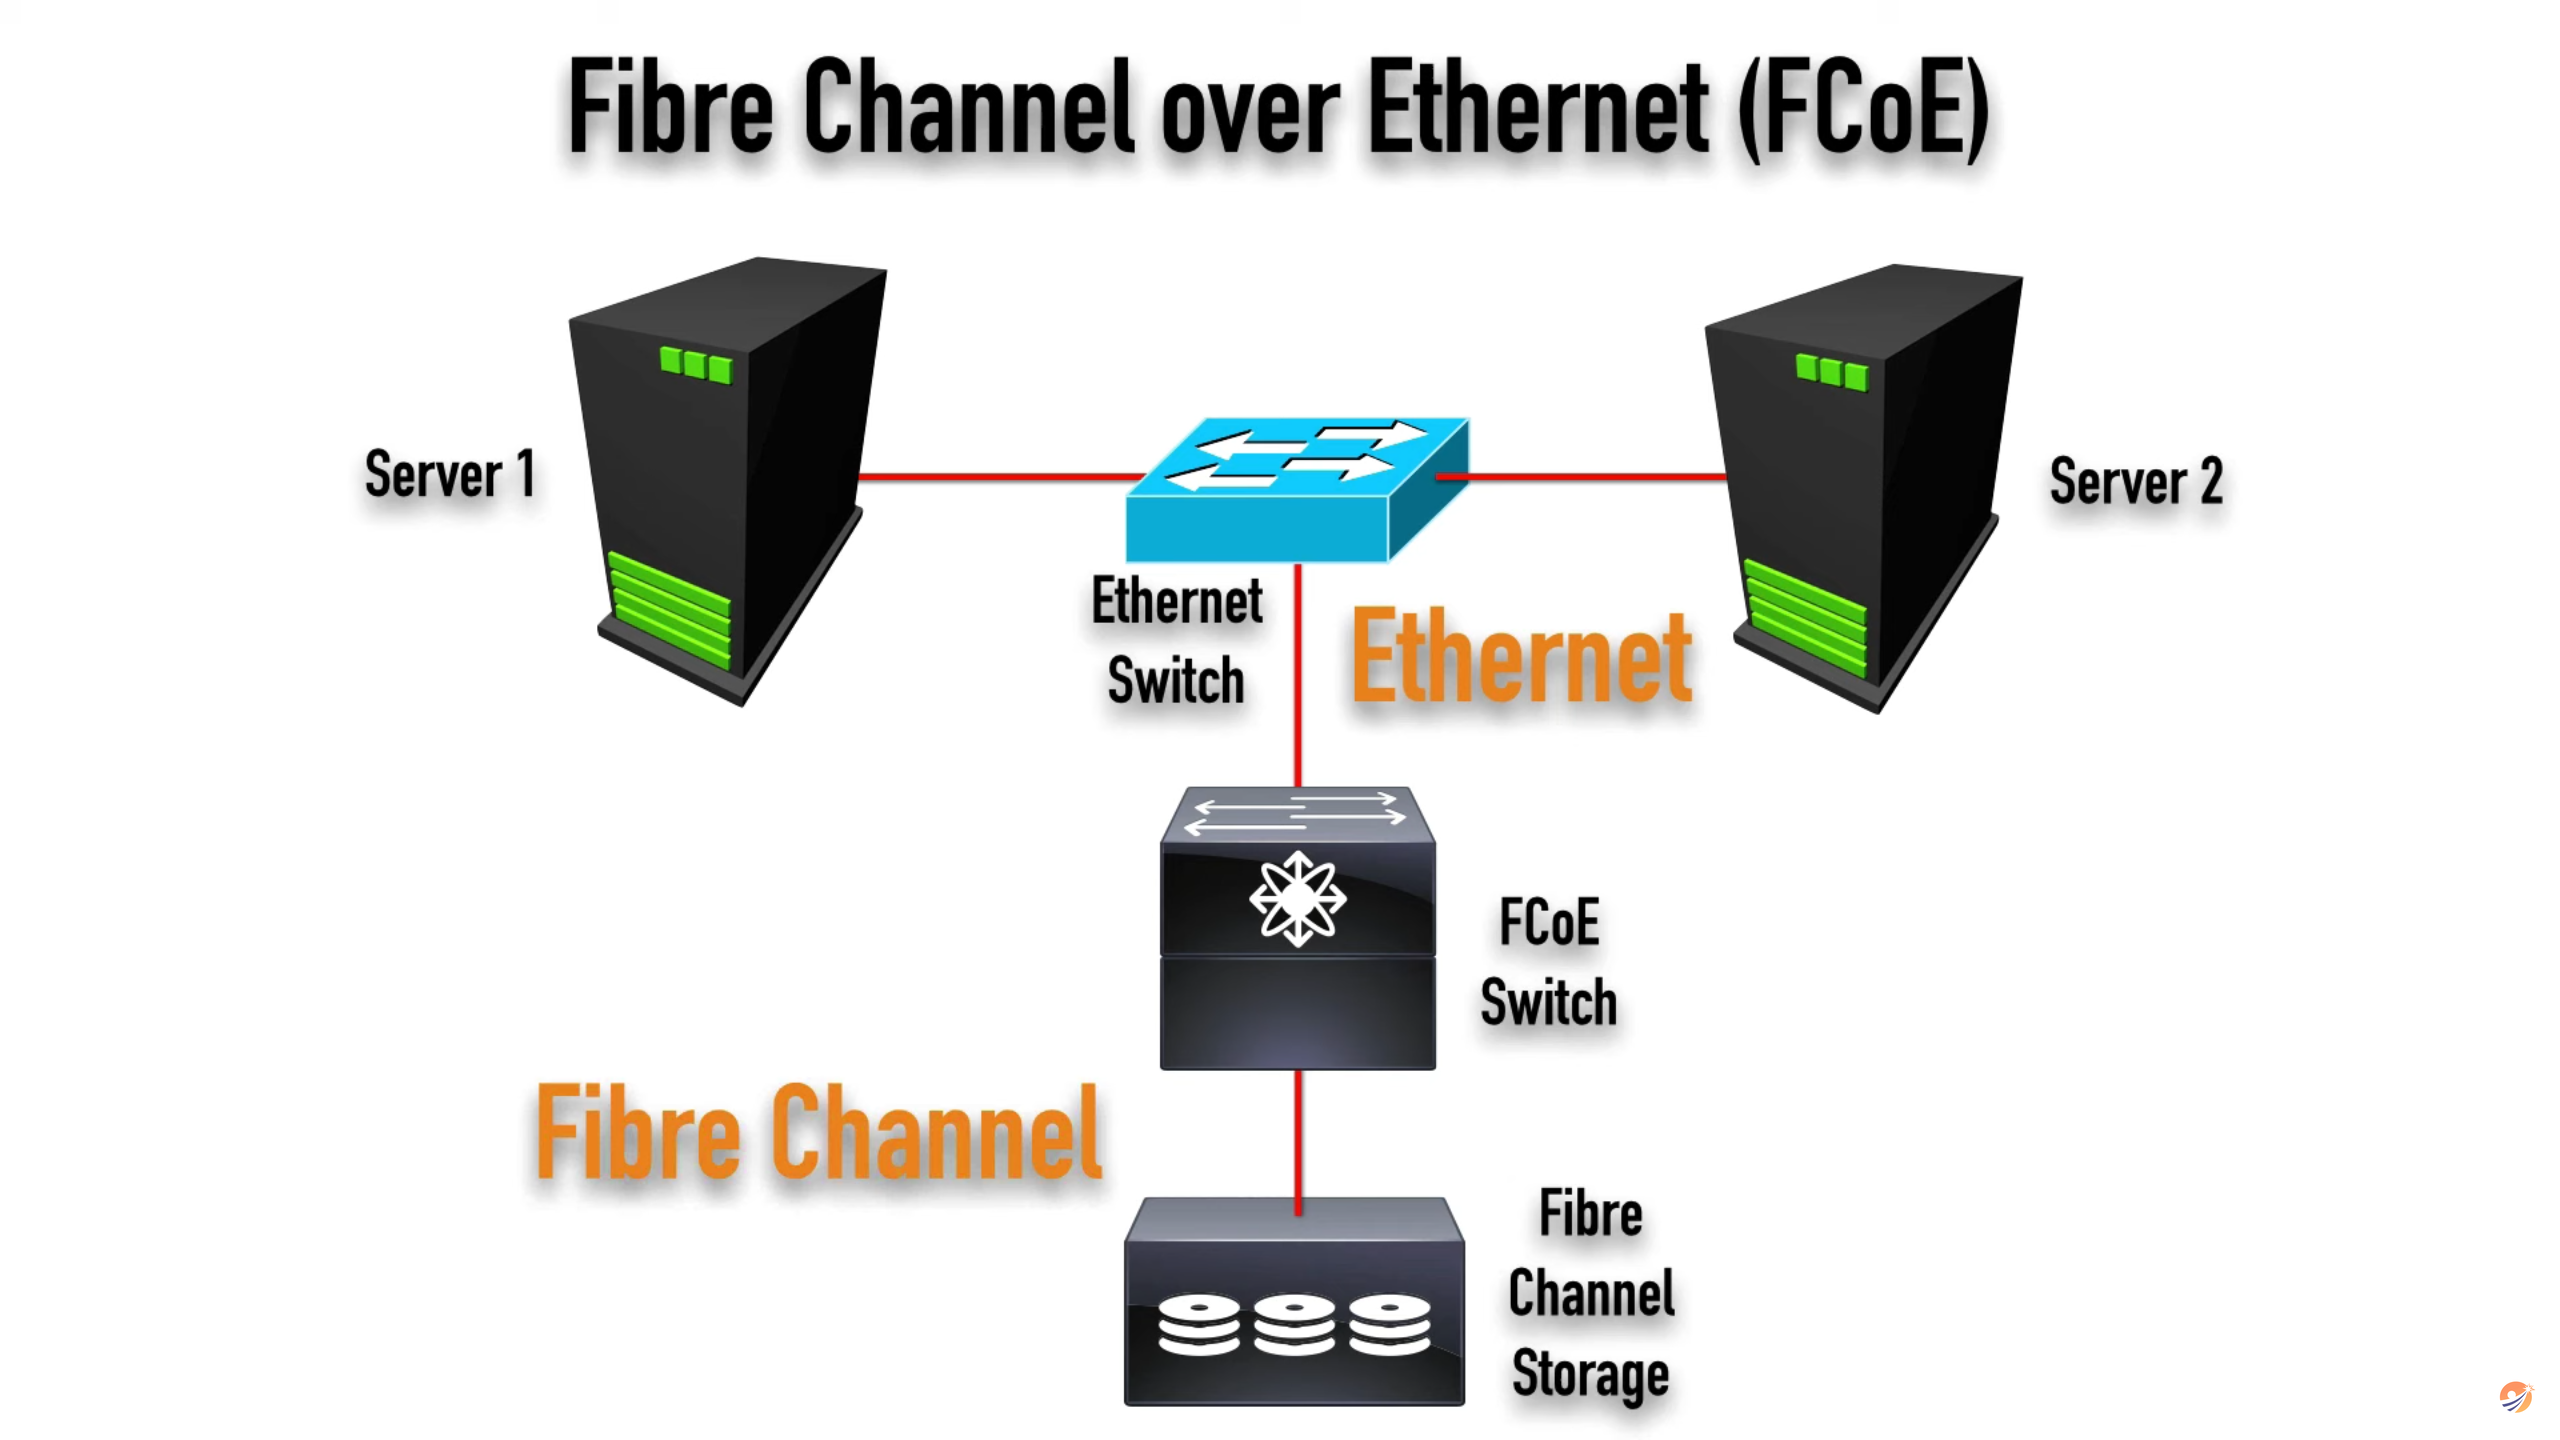
\includegraphics[width=0.32\columnwidth]{images/storage_fabric2.png}
   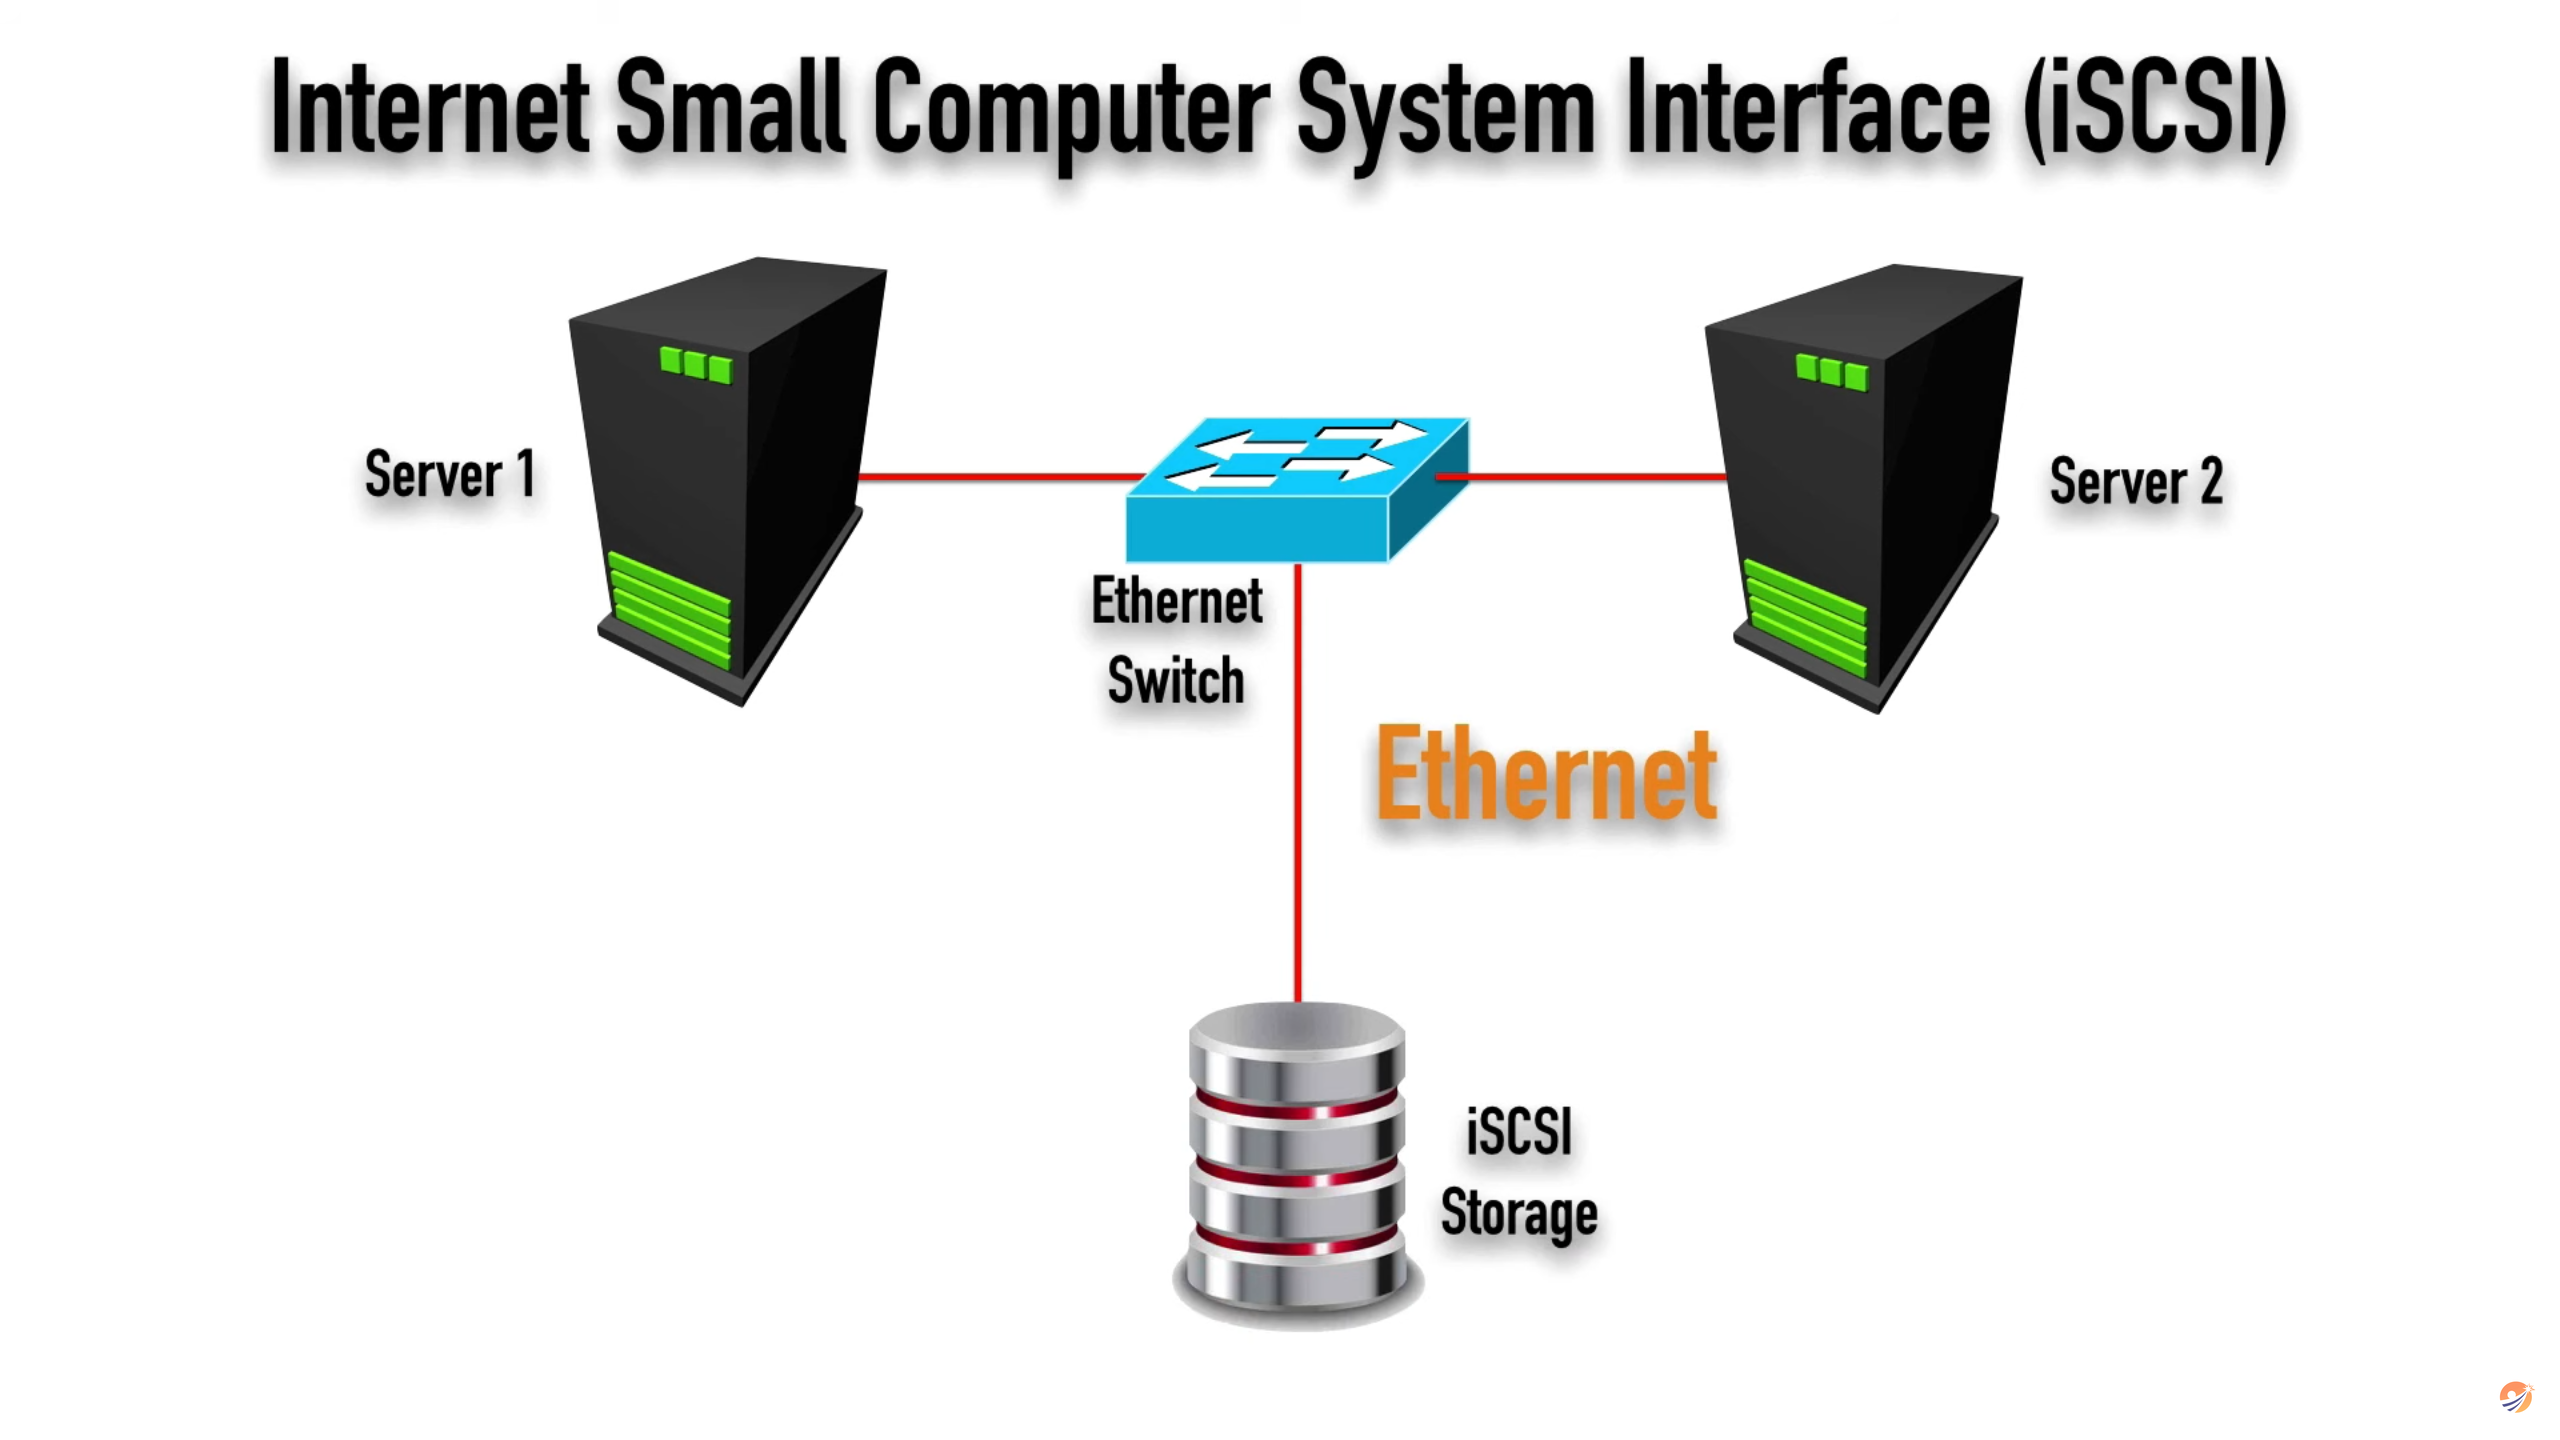
\includegraphics[width=0.32\columnwidth]{images/storage_fabric3.png}
   \caption{These are three possible configurations for the storage fabric, the first being the most performant, and the third being the cheapest.
   Note that in the second picture the first link is Ethernet and the second is Fibre Channel.}
   \label{fig:storage_fabric}
\end{figure}
Note that the image may me misleading, since there may be multiple FC switches (as partially depicted in Fig. \ref{fig:fibrechannel}) and multiple storage racks.
   
\subsection{Bus, controller and some numbers}
A bus is a component to whom multiple devices may be attached. It has a clock and some lanes, 16 in the case of PCI, each one providing almost 1GB bandwidth, summing up to $\sim 15GB$: 4 drives are enough to saturate a full PCI bus, or a 100Gbit link ($12.5GB/s$).;
in fact an NVMe SSD has a bandwidth of 3.5GB/s, hence $3.5\times 4 = 14GB/s \simeq 15GB/s$.\\
NVMe is often used in the lower memory tier of the RAM: its speed is only one order of magnitude less than RAM, but can provide high capacity without any problem.
It may represent a valid super-fast cache level for the RAM and hence started being associated in one single level to implement a big RAM tier, in a totally transparent way for the system.

Since the software latency in disk IOs is 5 microseconds more or less,
TCP/IP software introduces also a latency of 70-80 microseconds, the disk is
no more a problem. Indeed, the problem is now the network, not only for the
latency, but also for the bandwidth: as stated before 4 NVMe totally saturate a 100 Gbps
link.

\section{Redundancy and backup}
\subsection{Checkpoints}
It's unpractical for a system to go down after 5 months. For this reason it is necessary to have \ul{\textit{checkpoints}, which are points in time where the system can be restored to.} The system can be restored to the last checkpoint, and the data that was written after the checkpoint can be re-applied. This is similar to what happens to applications on smartphones are closed and then re-opened, the application is restored to the last checkpoint.

\subsection{RAID}
\textbf{RAID} stands for \textit{Redundant Array of Independent Disks}. It is a technology that allows to combine multiple disks into a single logical unit, in order to increase the performance, the reliability, or both. There are different levels of RAID, each with different characteristics.

Historically \textit{Redundant Array of Inexpensive Disks}, because it was more common for disks to eventually fail, so RAID was the only countermeasure to this. Today, disks are more reliable, so RAID is used more for performance reasons.

In RAID, \textbf{XOR} is used to calculate the parity of the data. The parity is used to recover the data in case of a disk failure. The parity is calculated by XORing the data of the disks. The parity is stored on a separate disk, called the parity disk. The parity disk is used to recover the data in case of a disk failure.


\section{Network sharing architectures}
Before going into the details of the architectures, it is important to understand the difference between \textbf{protocols} and \textbf{architectures}.\\
\textbf{SMB/CIFS} is a protocol that allows to share files over the network. It is used by Windows, but it is also supported by Linux and MacOS. NFS is a protocol that allows to share files over the network, it is used by Linux and MacOS, but it is also supported by Windows.\\
NFS is faster than SMB, but it is also less secure. SMB is slower than NFS, but it is also more secure.\\
These however are protocols for file sharing, not properly ``architectures''.

\framedt{Capacity and system architecture}{
   When we talk about \textbf{capacity}, there are two measures which we can refer to:
   \begin{enumerate}
      \item \textit{Scale-\textbf{up}}:
      adding more disks to the same server
      \item \textit{Scale-\textbf{out}}:
      adding more servers to the same network
   \end{enumerate}
}

\subsection{File based - NAS}
\textbf{NAS} are devices that are connected to the network, and that are used to store files, providing aggregated capacity. They are used to store files that are accessed by multiple users, and that need to be accessed from multiple devices.
NAS systems have integrated HW and SW component, including CPU, memory, NICs, optimized OS for file serving, file sharing protocols and so on.\\
Typically they exploit SMB/CIFS or NFS protocols, or AFP over optical fiber, and represent a good solution for \textit{document management}.

\subsection{Block based - SAN}
\textbf{SAN} stands for \textit{Storage Area Network}, which enables the creation and assignment (i.e. access and share) of storage volumes to compute systems.\\
The compute OS (or hypervisor) discovers these storage volumes as local drives.
The servers have different NICs (HBA) connected (usually through
fibre channels) to those blocks, which are aggregated volumes.\\
SAN also enables performance optimization of the storage by performing
deduplication (delete sequence of blocks that are equivalent).

\note{HBA stands for \textit{Host Bus Adapter}, and is a device that allows to connect a computer to a storage device. It is used to connect a computer to a storage device, and to allow the computer to access the storage device.}

SAN are a network separate from the LAN, so not affected by its traffic.\\
They usually exploit Fibre Channel or iSCSI (which is not as fast) protocols.

SAN was, before SSDs, one of the datacenter pillars.
Its architecture included a ``head'', an advanced Fibre Channel switch, to which drives were attached, and the head was connected to the network. The head was used to manage the drives, and to allow the servers to access the drives.\\
When SSDs became popular, the head became a bottleneck, because it was not able to keep up with the speed of the SSDs(Recall that 4 SSDs are enough to saturate a 10Gbit link, See Sec. \ref{sec:bandwidth_storage}). 
For this reason, the head may be removed, with the drives connected directly to the servers. This is called \textbf{DAS}, typically uses SCSI protocol, but is not as scalable as SAN.

However with groups of mechanical drives, ---if the data is splitted in a smart way--- it's possible to be faster of a single SSD, since the request will be forwarded in parallel to different drives.

\subsubsection{Protocols}
SANs are classified based on protocols and fabric they support. Some possible configurations can be found in Fig. \ref{fig:storage_fabric} 
Common SAN deployments types are Fibre Channel SAN (FC SAN), Internet Protocol SAN (IP SAN), and Fibre Channel over Ethernet SAN (FCoE SAN), ATA over Ethernet (AoE) and HyperSCSI ().
It can be implemented as some controllers attached to some JBoDS (Just a Bunch of Disks).

\note{While NAS provides both storage and a file system, SAN provides only block-based storage and leaves file system concerns on the “client” side.
However, note that a NAS \textit{can} be part of a SAN network.}


\subsubsection{Pools and LUNs}

\textbf{Storage pools} are used to combine multiple storage devices into a single logical unit, in order to increase performance and reliability. 

The SAN is divided in different Logical Unit Numbers (\textbf{LUN}s), which abstract identity and internal functions of storage devices, and appear as phyisical storage to the compute system.\\
\textbf{Storage LUNs} define a storage partition and are used to assign storage ---a portion of the pool--- to a server, and to allow the server to access the storage, using ACLs.
\nl

In the following section, some LUNs features are listed
\begin{itemize}
   \item 
   Storage \textbf{capacity} of a LUN can be dynamically expanded or reduced
   by means \textbf{virtual storage provisioning}, i.e. present a LUN as if it has more capacity than it actually has, to avoid fragmentatation and then expand it when it is needed.
   \note{e.g. if you assign a 1TB LUN to a server, and then you need to expand the LUN due to lack of space, if you have space next to the already assigned TB you can avoid fragmentation. Besides, if you can put data in only 1TB instead of 2TB (even if you present the volume as if it had 2TB), internal fragmentation may happen only inside that TB, and later on you can expand the volume up to the reserved 2TB.}
   Besides, \ul{available space may \textit{decrease} over time}, mostly due to snapshots (discussed later on).
   \item LUNs may perform \textbf{deduplication} (delete sequence of blocks that are equivalent/redundant, and exploiting indexes to retrieve duplicated data) to optimize storage performance. It is very useful in document-rich file systems, since people tend to copy a document multiple times.
   \item LUNs may perform \textbf{compression} to reduce the size of the data, and to increase the performance. It may be lossy or lossless.  Its major downside is that it is computationally expensive, since the data must decompressed before using it.
   On the other hand, allows to spare bandwidth by sending compressed data, which we know to be critical.\\
   \textit{Searching} in compressed data is not trivial, but there are tools to do it, such as the \href{https://en.wikipedia.org/wiki/FM-index}{\texttt{FM-index}}.
   \item LUNs may create \textbf{snapshots}, \textit{``point-in-time''} copy of current data state, to save the differences between the current state of the data and the previous state of the data. This allows to recover the overwritten data in case of a failure, but it also takes up space.\\
   Snapshots older than a week are usually deleted, since they are not needed anymore.
   
\end{itemize}

\subsubsection{Provisioning and Capacities}
LUNs may be created from\ns
\begin{itemize}
   \item A \ul{RAID set} (traditional approach); suited for application that require predictable performance
   \item A \ul{storage pool} (modern approach); suited for application that require flexibility and scalability, and that tolerate performance variations.
\end{itemize}

Both of these approaches have different capacities:\ns
\begin{itemize}
   \item Row capacity: the total capacity of the LUN, limited by the physical capacity of the storage devices
   \item Usable capacity: the capacity that is available to the server, limited by data structures needed to allocate the file system.
   \item Provisioned capacity: the capacity that you present to the server. May be more than the usable capacity, obtaining overprovisioning. 
\end{itemize}

\subsection{Object based - S3}
\textbf{S3} stands for \textit{Simple Storage Service}, and is a service that is used to store file data in the form of objects based on the content and other attributes of the data rather than the name and location of the file.
The additional metadata (size, date, ownership\dots) or attributes (retention, access pattern\dots) enable optimized search, retention and deletion of objects.\\
A flat, non-hierarchical address space to store data provides the flexibility to \textit{scale massively}.\\
\ul{S3 is leveraged to provide Storage as Service.}

\subsection{Big Data - HDFS}
\textbf{HDFS} stands for \textit{Hadoop Distributed File System}, and is a distributed file system that is used to store large amounts of data across multiple servers.
A \texttt{map/reduce} algorithm is applied on the data, and then results are collected and summarized.\\
It exploits good forms of parallelism to run efficiently the algorithm

\subsection{Unified - Unified Storage}
\textbf{Unified Storage} or multi-protocol storage has emerged as solution that consolidates block, file and object storage into a single storage platform. It supports multiple protocols, such as NFS, SMB, iSCSI, FC, REST and SOAP.

\framedt{iSCSI and its death}{
   SCSI (Small Computer System Interface) was invented in 1979 for chaining drives
   through a bus (used for e.g. in fibre channels). The controller was so smart
   to allow the the drive to share the flat cable as a bus.\\
   Over the time some variants were invented, but the basic idea is the same.
   One example is iSCSI: \textit{Internet Small Computer Systems Interface}, an IP-based storage networking standard for linking data storage facilities.
   It provides block-level access to storage devices by carrying SCSI commands over a TCP/IP network. The protocol died when SSD were introduced, since the latency was too high when communicating over the network.

   The key idea behind SCSI was for \ul{mutiple drives to share the same physical flat cable}.\\
   It had been ``deprecated'' in favor of \texttt{NVMe}, but it is still used today, because it is very reliable.
}
\subsection{Synchronization Software and its Price}
The ``storage guy'' must ensure that there is no condition under which can happen data loss, because it is never an option. It is also important to have powerful \textbf{synchronization algorithms}, which must allow data to be copied and synchronized in multiple locations without disrupting performance and handling concurrency;
such software is typically \textit{costful}.

It is difficult nowdays to establish what is the ``right'' price for software. The shift from highly specialized and costful hardware to general hardware-plus-software, gave the software, which still is a non-physical entity, increasingly more value, perhaps even too much.


\section{Hyperconverged Infrastructure}
SAN started to create a sensible bottleneck, so designers started to ``move drives towards the servers''.
\textbf{DAS} stands for \textit{Direct Attached Storage}, and is a technology that allows to connect multiple storage devices to a single server, in order to increase the performance, the reliability, or both.
The limitations is that you can only attach up to 2 or 3 drives to a server.

An idea came out to use the servers' internal drive to build a Storage Area Network, and this is called \textbf{VSAN}.

\subsection{HCI solutions}
\textbf{HCI} stands for \textit{Hyperconverged Infrastructure}, and is a technology that allows to combine multiple servers into a single logical unit, in order to increase the performance, the reliability, or both. 
The idea was born to allow a scale-out architecture, where you can add more servers to the network.

\begin{center}
   \ul{\textit{``Adding servers adds capacity''}}
\end{center}

The \textbf{Hypervisor} is the software that allows to run multiple virtual machines on a single server. There should be some locality between the VM and the storage, because the VM should be able to access the storage quickly.\\
The \textit{controller VM} (one per host) implements the storage abstraction and the logical moving of data.
\texttt{read} operations are always performed locally on local drives; \texttt{write} operations instead sometimes require to retrieve a remote piece of data.
A copy on the local server storage is kept, but the server needs to wait for the acknowledgment of the remote server in order to keep updated replicas of written data in other nodes.

As mentioned in the section dedicated to HCI and networking Sec. \ref{sec:HCI_network}, new server are automatically added to the network seamlessly integrating with the pre-existing HCI cluster.
The same applies to the storage, which is automatically added to the pool, and local replicas of data are built.

\subsubsection{VM Live Migration}
Live Migration of VMs is a technique that allows to move a VM from one server to another server, without interrupting the service. 
When it happens over SAN there's no need to copy storage to the new server, since the storage is shared and accessed through the network.
The case of HCI is similar since the storage is mostly shared, but there are also the above mentioned local copies of data, which may need to be updated. 

\subsection*{Riak and Acropolis}
Riak is a distributed database that is used to store data in multiple locations. 
The same applies to Acropolis, which is a distributed storage system.

Recently it has been recognized that \ul{using general purpose hardware is no longer a feasible option.}

\section{SDS - Software Defined Storage}
\textbf{SDS} \textit{Software Defined Storage} refers to software for policy-based provisioning and management of data storage independently from the underlying hardware.
Such software is more costful than the hardware it is running on, since it also optizimes the drives, not simply managing them.\\
SDS exploits object-based storage architecture and DHTs to provide storage services.